%\chapter{Introducci\'on} % (fold)
%\label{cha:introduccion}
%\addcontentsline{toc}{chapter}{Introducción}

\section{Contexto}

En el nuevo ambiente de las tecnologías de la información se encuentran los usuarios de estas tecnologías y las organizaciones, cualquier movimiento de almacenamiento masivo computacional puede ser realizado mediante modelos  basados en el cómputo nube. Asimismo, al manejar un gran volumen de información, los usuarios buscan la posibilidad de que al almacenar esos datos, puedan ser accedidos a ellos de manera fácil y desde cualquier ligar o dispositivo en donde han accedido los usuarios ~\cite{Nubei}. \\ \\ 

Según un estudio realizado por Computerworld (una revista mundial reconocida por su enfoque a las tecnologías de la informaión y comunicación) a empresas de tecnologías de la información, aseguran que el 42\% de estas empresas de TI están planeando aumentar el gasto en Cloud Computing (Cómputo nube), siendo el crecimiento mayor en las empresas con más de 1000 empleados (52\%). Las 5 áreas de mayor crecimiento se ilustran en la figura ~\ref{fig:1-1-1}

\begin{figure}[H]
\centering
	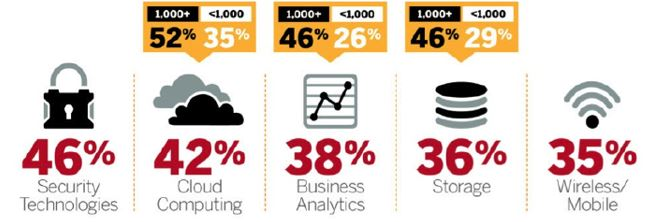
\includegraphics[width=15cm, height=5cm]{./images/aumentoCloudComputing.jpg}
	\caption{Aumento del gasto por las empresas en cómputo nube}
	\label{fig:1-1-1}
\end{figure}


El cómputo nube es un término general utilizado para nombrar así a la provisión de servicios de almacenamiento a través de internet que ha sido utilizado para facilitar el cambio de los modelos de negocios, agilizar procesos y reducir los costos de operación en las grandes empresas u organizaciones. Uno de los mayores beneficios que ofrece este servicio es la virtualización de los centros de datos, que pueden operar de manera automatizada, sin  necesidad de la presencia de una persona física y ser pueden ser gestionados en cualquier momento y tiempo. De acuerdo con un estudio realizado por la consultora Market Research Media, el cloud computing generará \$270,000 millones de dólares en 2020, por lo que empresas como Google, Amazon, IBM, Oracle y Apple han adoptado este sistema como parte del servicio brindado a sus consumidores, por ejemplo Google Drive o iCloud, a través de los cuales, con sólo estar conectados a Internet, los usuarios tienen la posibilidad de utilizarlos ~\cite{Nubecomp}. \\ \\ Básicamente el almacenamiento en la nube se caracteriza por 5 puntos esenciales que son: 
	\begin{itemize}
		\item \textbf{Autoservicio on-demand o pago por evento}  
		\item \textbf{Acceso ubicuo a la red (uso de los servicios cuando sea y donde sea)}  
		\item \textbf{Fondo común de recursos} 
		\item \textbf{Rápida elasticidad} 
 		\item \textbf{Servicio medido}  ~\cite{Compnube}.
 \end{itemize}

\section{Problemática}
Hoy en día el manejo de información en la sociedad juega un papel importante en el desarrollo de las actividades que la conforman. Millones de personas en el mundo tienen la facilidad de acceder a un dispositivo electrónico que les permite manipular esta información o almacenarla ya sea en un dispositivo físico o en algo más nuevo y eficiente como la nube, para posteriormente darle un uso específico.
El cambio en las estrategias de negocio y la explosión de datos digitales se ha lanzado enormes demandas de alto volumen y almacenamiento de datos eficiente. Debido a los limitados recursos financieros y altos gastos de almacenamiento de datos electrónicos, los usuarios prefieren almacenar sus datos en los entornos de nube, el almacenamiento en la nube permite a sus usuarios transferir sus datos y aplicaciones en la web para que puedan operar esos programas sin ninguna infraestructura física necesaria ~\cite{Keelveedhi}.
\\
 Ahora bien, la información que circula en dispositivos electrónicos es mayor a la memoria disponible que ofrecen estos, a medida que el volumen de información aumenta, también lo hace la demanda para los servicios de almacenamiento en línea ~\cite{Bellare}. Un gran incremento en el uso de estos servicios implica tener más infraestructura y personal para que los sistemas de almacenamiento tengan más capacidad y puedan cubrir la demanda que se presenta en el mercado. Si bien el almacenamiento logró dar buenos resultados al cliente en sus primeras etapas, ahora la preocupación por el incremento de infraestructura para seguir dando esos resultados se ha incrementado considerablemente  ~\cite{Keelveedhi}.
\\ 

Para entender un poco más acerca de la problemática que se enfrenta el almacenamiento en la nube, mostramos el siguiente estudio realizado por EFE/Cisco:\\ 

EFE/Cisco realizó una estimación en el año 2014 en su cuarto informe anual Índice Global sobre Cloud (2013-2018), donde prevé que en 2018 la mitad de la población mundial tendrá internet en sus hogares y más de la mitad almacenará contenidos en servicios personales de almacenamiento en la nube. El estudio adelanta que se triplicará el crecimiento de tráfico en los centros de datos en los próximos cinco años y la nube representará el 76\% de ese total, mientras que en 2013 éste solo representaba el 54\%, lo que supondría un aumento anual de 32\%. El tráfico en centros de datos, contando el saliente a usuarios finales, entre centros y dentro del propio sistema, superará los 3,1 zettabytes de 2013 y llegará a los 8,6 que se esperan registrar en 2018, suponiendo una tasa anual del 23\% ~\cite{cisco}. 
\\ 
En 2018, el 53\% de los usuarios de internet con red doméstica usarán servicios de almacenamiento en la nube, aportando un tráfico medio por usuario de 811 mb mensuales, lejos de los 186 mb de 2013. Además se espera, según la nota de prensa, que en 2018 el 69\% de la carga de trabajo en la nube se realice en centros de datos con nubes privadas, un dato que fue del 78\% en 2013. El resto de cargas de trabajo, el 31\%, se realizarán en la nube pública, subiendo desde el 22\% del año pasado ~\cite{cisco}. Crecimiento en el tráfico de información el la nube ~\ref{fig:1-2-1} \\

\begin{figure}[H]
\centering
	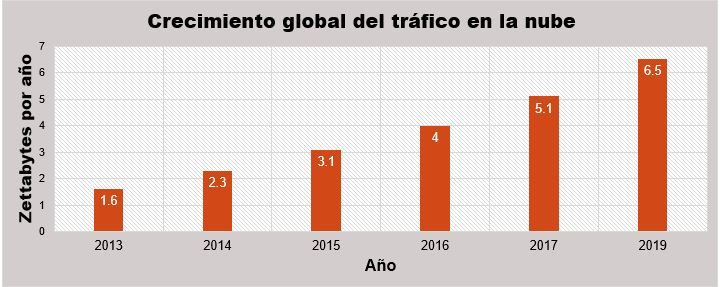
\includegraphics[width=13cm, height=5cm]{./images/crecimientoNube.jpg}
	\caption{Crecimiento global del tráfico en la nube}
	\label{fig:1-2-1}
\end{figure}

Una de las principales razones del incremento en el tamaño en la estructura de almacenamiento de servicios en linea es la duplicación de archivos por varios y diferentes usuarios, existen muchas copias en la nube de un mismo archivo que se encuentra presente en diferentes cuentas de usuarios. Por ejemplo \textbf{\textit{n}}cantidad de  usuarios pueden subir la misma canción a la nube, por lo tanto esta se encuentra almacenada en las \textbf{\textit{n}} cantidad de cuentas que tiene registro la nube, esta misma canción que se encuentra almacenada está cubriendo un espacio en la memoria del servicio, si se tuviera una sóla copia almacenada de esta canción se ahorraría mucho espacio en la nube que podría utilizarse para el aalmacenamiento de un archivo diferente . Según un estudio ~\cite{popa} realizado por HP se estima que hay 1 Exabyte de datos almacenados en la nube, además de 2012 a 2017, las cargas de trabajo de los centros de datos crecerán 2.3 veces, mientras que en la nube aumentarán 3.7 veces, lo cual implica que el Exabyte que se estima se podría llegar a triplicar y las empresas que proporcionan estos servicios disminuyen su oferta en el mercado. 
\\ 
Otro punto importante 
%Sumado al agraviante problema de crecimiento en la estructura de almacenamiento en línea, existe un elemento que pocas organizaciones y usuarios contemplan para el almacenamiento de su información, y es la seguridad. Las plataformas que ahora ofrecen el servicio de almacenamiento en la nube, no contemplan la protección e integridad de la información, este servicio está sujeto a los ataques de adversarios que están interesados en el robo, manipulación o alteración de la información importante para los usuarios. Dicho servicio carece de algún esquema de seguridad y por tanto no se puede garantizar la permanencia de los usuarios en el consumo del servicio en la plataforma de almacenamiento. 
%Dejar sin resolver la seguridad de la infofrmación, puede generar negativas consecuenicias hacia cualquier usuario de la plataforma de almacencamiento, cualquier individuo que tenga acceso a los archivos almacenados en ésta plataforma, podrá visualizar el contenido de estos, comprometiendo la fidelidad e integridad de la información para poder usarla en situaciones que pudieran llegar a perjudicar al usuario. 
\\

\section{Estado del Arte}
\begin{tabular}{ |p{3cm}|p{2.5cm}|p{2.5cm}|p{2.5cm}|p{2.5cm}|p{2.5cm}|p{2.5cm}| }
\hline
\multicolumn{5}{|c|}{APLICACIONES}\\
\hline
{}  & {DupLESS } & {TahoeFS } & {Flud Backup} & {ABS: The Apportioned Backup System} \\
\hline
{ Evitar duplicación de archivos}  & {Si} & {No} & {No} & {Si}  \\
\hline
{Seguridad al cliente}  & {Alta} & {Media} & {Media} & {Alta}  \\
\hline
{Resistencia a ataques por fuerza bruta}  & {Si} & {Media} & { No} & {No}  \\
\hline
{Compromiso de resistencia ante fallos}  & {Alto} & {Alto} & {Alto} & {Alto}  \\
\hline
{Privacidad}  & {Si} & {Si}  & {No} & { Si }  \\
\hline
{Servidor Seguro}  & {Si} & {Si} & {Si } & {Si} \\
\hline
{Implementación }  & { Pruebas } & {Actualmente Operacional} & { Actualmente Inactivo } & {Pruebas }  \\
\hline
{Código abierto}  & {Si} & {Si} & {Si} & {No}  \\
\hline
{Gratuita o de paga}  & {Sin información} & {Ambos} & {Gratuito} & {Sin información} \\
\hline
\end{tabular}

\begin{itemize}
\item DupLESS\\
Este protocolo usa un servicio de almacenamiento en la nube, además implementa una interfaz sencilla con operaciones como guardar, recuperar o borrar un archivo. Es más adecuado para aplicaciones backup y busca proteger la confidencialidad de datos de los clientes, para ello usa seguridad semántica. Además promete capacidad de resistencia ante fallos, protección contra un servidor malintencionado, evitar duplicación de archivos y compatibilidad con diferentes sistemas operativos~\cite{Bellare}.
\item TahoeFS\\
Este sistema utiliza diez diferentes servidores que se interconectan entre sí y consta de archivos mutables e inmutables. Se basa en la restricción a los usuarios de cierto comportamiento. A los archivos mutables les permite operaciones como leer y verificar y a los inmutables les permite leer, escribir y crear copia de solo lectura. Hace uso de cifrado convergente, el código Reed-Solomon para la tolerancia a fallos, el servicio AllMyData y control de acceso descentralizado.
Es un servicio que promete almacenamiento seguro, integridad y confidencialidad a largo plazo y va enfocado a aplicaciones backup~\cite{tahoe}.
\item Flud Backup\\
El proyecto Flud Backup está actualmente inactivo, sin embargo se crearon diversas versiones para Ubuntu y Fedora donde usan paquetes distribuidos y un sistema de confianza. Prometen que los datos que se copian deben ser indestructibles y copias de seguridad descentralizadas~\cite{flud}.
\item ABS\\
Este sistema se centra en el caso de uso de diez PC's conectadas a través de una LAN o a través de conexiones de Internet de Banda Ancha.Se basa en el almacenamiento de fragmentos y algo que denominan 'almacén de instancia única' donde si dos usuarios almacenan el mismo contenido del archivo, el sistema generará los fragmentos independientes de cada archivo y solamente almacenará una copia de cada fragmento en la red. También tiene un esquema de asignación de versione basada en rsync (para generar una firma de diferencia sobre el archivo, la cual es una representación compacta, basada en el hash de un archivo que permita comparar entre dos versiones de archivos y verificar si están duplicadas. 
Promete el almacenamiento de datos seguro y eficiente, privacidad y seguridad, esto a través de tablas hash distribuidas, firmas de clave privadas, control de versiones y cifrado convergente. 
Además es tolerante a fallas catastróficas a nodos y permite unir nodos y restaurar operaciones sin pérdida de datos~\cite{abs}.
\end{itemize}

\section{Justificación}

En la actualidad millones de personas usan los servicios de almacenamiento que ofrece la nube, ya sean gratuitos o privados, este número de personas ha ido en un incremento exponencial lo cual hace que el espacio de almacenamiento disminuya, entonces ¿Cómo podría mitigar el problema de almacenamiento y tener privacidad de los datos al mismo tiempo?

Usando la criptografía clásica para poder cifrar un archivo se utiliza una clave privada la cuál es distinta para cada usuario, cada vez que se cifra un archivo el resultado de este es diferente para cada intento. Por tanto no se puede evitar la duplicación de archivos utilizando este mecanismo de la criptografía y se deben implementar soluciones más robustas.

Una solución para tener privacidad y evitar duplicación la proporcionó John R. Douceur, la cual dice que teniendo a M que será el contenido de un archivo de aquí en adelante denominado el mensaje, el cliente primero calcula una clave K ← H(M) mediante la aplicación de una función de hash criptográfica H al mensaje y luego calcula el texto cifrado C ← E(K,M) a través de un esquema de cifrado simétrico determinista. El derivado del mensaje K se almacena por separado cifrándolo con una llave por cliente. Un segundo cliente B cifra el mismo archivo M que producirá el mismo C, evitando la duplicación. ~\cite{donceur}

En el artículo publicado por Mihir Bellare, Sriram Keelveedhi, Thomas Ristenpart, nombrado “DupLESS: Server-Aided Encryption for Deduplicated Storage” ~\cite{Bellare}, se observó que uno de los principales problemas al que nos enfrentamos es que el esquema de cifrado solo es seguro cuando el espacio de mensajes es demasiado grande, por lo tanto agentes externos pueden provocar agravios a la integridad de la información de los usuarios.

Si bien esta solución se ocupa de la duplicación de archivos deja muy vulnerable el aspecto de la privacidad, ya que ante un espacio de mensajes pequeño las amenazas del adversario son demasiadas. Si se tuvieran como ejemplo 1000 mensajes, para el adversario sería muy fácil intentar encontrar la clave, probando las 1000 claves posibles generadas con la función hash, hasta descifrar el archivo, por lo tanto se comprueba que un espacio de 1000 mensajes sigue siendo pequeño.

Es por ello que este trabajo terminal tiene como principal meta atacar esta problemática de privacidad, proponiendo una arquitectura del sistema que a través de un servidor de llaves se generaran llaves de acuerdo al contenido del archivo, para con esta se pueda cifrar y luego almacenar en la nube donde se eludirá la duplicación de archivos. 



\section{Solución propuesta}
La eliminación de duplicación de datos es una experiencia progresiva que puede disminuir drásticamente la cantidad de información de respaldo almacenada eliminando todos los datos redundantes como se ilustra en la figura ~\ref{fig:1-3-1}. Al evitar la duplicación de datos explota el consumo de almacenamiento mientras que permite a las tecnologías de información recuperar más datos de respaldo de líneas cercanas durante más tiempo. Esto recupera enormemente la capacidad del disco de copia de seguridad establecida, alterando la forma en que los datos están protegidos. En general,
la eliminación de duplicados compara la información nueva con la información actual de los trabajos anteriores de copia de seguridad o archivado y elimina las redundancias en la nube reduciendo la asignación de almacenamiento dentro de esta, puede reducir las necesidades de almacenamiento en hasta un \textit{80\%} para archivos y copias de seguridad que los usuarios resguardan en la nube. Las ventajas de no tener duplicados en la nube incluyen una mayor capacidad de almacenamiento y ahorro presupuestario, al igual que la minimización del ancho de banda para menos costosa y más rápida la repetición de la información fuera de la reserva simplificando y mejorando la gestión del almacenamiento de datos  ~\cite{rededup}. 


Una posible solución para la protección a los datos y eliminar duplicaciones de estos, es echar mano de la criptografía. Ciencia que se encarga del estudio de técnicas para transformar la información a una forma que no pueda entenderse a simple vista; sin embargo, el objetivo de la Criptografía no es sólo mantener los datos secretos, sino también protegerlos contra modificación o manipulación y comprobar la fuente de los mismos ~\cite{fundamentos}. \\   
Está ciencia que matiene la información segura se encuentra dividida en dos grandes tipos: \textbf{Criptográfia simétrica} y la \textbf{Criptografía asimétrica}.  
\begin{itemize} 
   \item \textit{La criptografía simétrica} o también llamada criptografía de llave privada, basa su seguridad en una sóla llave que se comparte entre dos usuarios que quieren compartir información, dicha llave es utilizada para cifrar un archivo al ser enviado al otro usuario y este utilizará la misma llave para descifrarlo cuando lo reciba. 
\item \textit{La criptografía asimétrica} o criptografía de llave pública involucra el uso de un par de llaves para cada usuario que desea comunicarse, estas llaves llamadas pública y privada. Para que un usuario envíe un archivo a otro usuario necesita cifrar el archivo con la llave pública de ese usuario al que se desea enviar, y cuando lo reciba ese usuario lo deberá descifrar con su llave privada o secreta. De esta manera se evita el compartir llaves para cifrar y descifrar como sucede en la criptografía simétrica y reduce los riesgos de un ataque de adversarios. 
 \end{itemize}

El objetivo de esta propuesta de solución es almacenar más datos en menos espacio mediante el uso de la criptografía. Esta ciencia nos proveerá con sus herramientas para la creación de un llavero criptográfico, dicho llavero realizará una firma la cuál dará paso a la creación de una llave correspondiente a un archivo \textit{F} que se desee almacenar un usuario, si se llega a solicitar al llavero por un usuario diferente una nueva firma para la creación de una llave para el mismo archivo \textit{F}, esta llave será la misma, ya que el mecanismo de funcionamiento entre un usuario y este servidor está diseñado para que sea capaz de identificar el mismo archivo sin comprometer el contenido e integridad de este. Esta  llave va a lograr que cuando se cifre este archivo por \textit{n} cantidad de usuarios diferentes que lo poseen, dicho cifrado será igual para la \textit{n} cantidad de usuarios, permitiendo así que en la nube al subir estos cifrados se realice una comparación para que reconozca a quien pertenecen esos cifrados y sólo tenga almacenada una sola copia de este, ahorrando espacio de memoria y costos de infraestructura. 

\begin{figure}[H]
\centering
	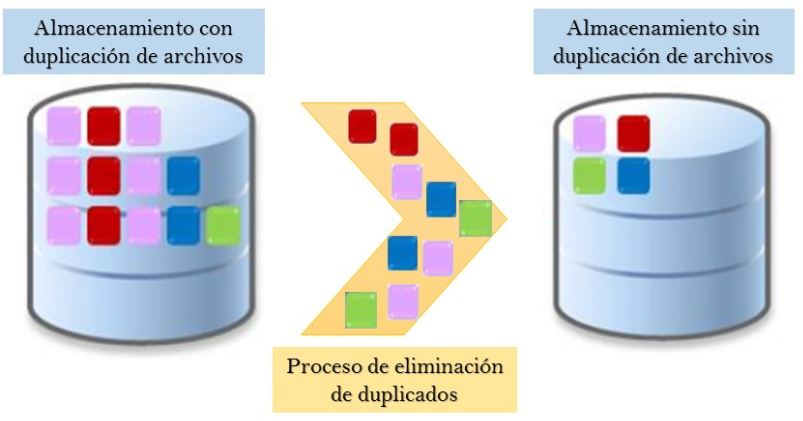
\includegraphics[width=10cm, height=5cm]{./images/Deduplicacion.jpg}
	\caption{Solución Propuesta}
	\label{fig:1-3-1}
\end{figure}



Puesto que ambas cuestiones, la eliminación de duplicados y la privacidad de la información, son importantes, se ha comenzado a
proponer mecanismos que solucionen ambos problemas de manera conjunta, que son: Dupless ~\cite{Bellare}, ABS: the apportioned backup
system. ~\cite{abs}, Flud Backup ~\cite{flud}, SIGOPS Oper. Syst. ~\cite{sigops}, TahoeFS ~\cite{tahoe}.


\section{Objetivos} % (fold)

    \subsection{Objetivo General} % (fold)
    Desarrollar un protocolo criptográfico para evitar la duplicación de archivos almacenados en la nube, garantizando la privacidad de los usuarios contra adversarios cuando el espacio de mensajes es pequeño, utilizando algoritmos criptográficos para su implementación. 
     
    \subsection{Objetivos Específicos} % (fold)
	\begin{itemize}
		\item Evitar la duplicación de archivos que sean almacenados por los usuarios de la nube
		\item Proteger ante los adversarios la información de los usuarios de la nube
		\item Establecer un esquema de autenticación de usuarios 
		\item Reducir la pérdida y filtración de información de los usuarios de la nube
		\item Evitar los ataques por fuerza bruta al contenido de los archivos de usuarios en la nube. 
 	\end{itemize}
    